\chapter[Clustering Uncertain Data Based on GLD Similarity]{Clustering Uncertain Data Based on GLD Similarity}\label{cap:gld_clustering}

In chapter \ref{cap:gld} we exposed the two most important parametrizations of the \textit{GLD} and select the \textit{FMKL} as  the one to use for the rest of the  thesis. In this parameterization $\lambda_{1}$ represent the location of the \textit{GLD} and is directly related to the mean of the distribution. $\lambda_{2}$ is the scale, directly related to the standard deviation; and $\lambda_{3}$ and $\lambda_{4}$ represent the left and right tails of the distribution. Combinations of $\lambda_{3}$ and $\lambda_{4}$ can be used to estimate the skewness and kurtosis of the distribution.

The uncertainty can be characterized in many different ways as we mention in chapter \ref{cap:backgroud}, but from the \textit{GLD} point of view, $\lambda_{2}$, $\lambda_{3}$ and $\lambda_{4}$ are the responsables of this. So, in this chapter we try to answer the research question 1, we formulate in the introduction:

\begin{tcolorbox}
\textbf{RQ1.} how to group the output of the UQ process based on the similarity of the uncertainty?
\end{tcolorbox}


First of all, in section \ref{sec:related_works} a brief review of some related works is performed. In this section, some advantage and drawbacks are highlighted, and some considerations about the possibilities of the use of the \textit{GLD} to solve some of the drawbacks are commented. Next, in section \ref{sec:clustering_gld} our hypothesis about the use of the \textit{GLD} to clusterized uncertain data, is presented. Sections \ref{sec:synthetic_I} and \ref{sec:synthetic_II} present two synthetics datasets and the results of the clustering technique. Those results help us to validate our hypothesis. Finally, section \ref{sec:conclusions} summarize and discuss the main results of the chapter.

\section{Related Works}\label{sec:related_works}

\cite{Jiang2011}

\section{Clustering Based on GLD}\label{sec:clustering_gld}

Our hypothesis is that, as the \textit{GLD} shape is characterized by $\lambda_{2}$, $\lambda_{3}$ and $\lambda_{4}$, and this shape change slowly with the change in the $\lambda_{i}$  values, we can group the uncertainty using clustering algorithms above $\lambda_{2}$, $\lambda_{3}$ and $\lambda_{4}$.  

To test our hypothesis, we generate two synthetic datasets using 4 different probabiltiy density functions: Gaussian, Exponential, Uniform and Gamma. The structure of the datasets is represented in \ref{eq:multi_array}.  

\begin{equation}\label{eq:multi_array}
S(x_{i}, <v_{j}>) i=1.....n,j=1.....m
\end{equation}

where:
\begin{itemize}
\item n represent the number of objects of the dataset and,
\item m represent the size of each object.
\end{itemize}

For example, the first object could be a Gaussian distribution with size = 1000, mean = 0 and standard deviation = 2, figure \ref{fig:normal_sample}. The datasets are described in details in sections \ref{sec:synthetic_I} and \ref{sec:synthetic_II}. 

%Independently of the dataset, the first step is to fit the \textit{GLD} to each distribution. In the next subsection we present the algorithm used to do this.

\subsection{Fit the GLD to a dataset}\label{sub:fitting_gld}
When we generate a synthetic dataset, the next step is to find the \textit{GLD} that best fit $<v_{j}>$ on each $x_{i}$. As the fitting process is computationally intensive we implement a parallel algorithm using \textbf{R}. The seudo-code is shown in algorithm \ref{alg:fitGLDSyntheticDataset}.

\begin{algorithm} 
\caption{Fitting the GLD to a synthetic dataset}\label{alg:fitGLDSyntheticDataset}
\begin{algorithmic}[1] 
\Function{gldFit}{$S(x_{i},<v_1,v_2,...,v_{n}>)$} 
\State $<\lambda_{1},\lambda_{2},\lambda_{3},\lambda_{4}> \gets \Call {fit.gld.lm}{<v_1,v_2,...,v_{n}>}$

\State $isValid_{(x_{i})} \gets \Call {validityCheck}{<\lambda_{3},\lambda_{4}>}$
\If{$isValid_{(x_{i})}$}
\State $[pvalue,D]_{(x_{i})} \gets \Call{ks}{<\lambda_{1},\lambda_{2},\lambda_{3},\lambda_{4}>_{(x_{i})}}$
\EndIf
\If{$pvalue_{(x_{i})} > 0.05$}
\State $\Call{storeLambdas}{<\lambda_{1},\lambda_{2},\lambda_{3},\lambda_{4}>,x_{i}}$
\EndIf
\EndFunction 
\end{algorithmic} 
\end{algorithm} 

The algorithm receive a dataset represented by \ref{eq:multi_array} and, for each position $x_{i}$, call a function \textbf{\textit{fit.gld.lm}} from the \textbf{R} package \textbf{GLDEX} presented in section \ref{sec:gldex}, line 2 of the algorithm \ref{alg:fitGLDSyntheticDataset}. In line 3 we check the validity of the \textit{GLD} returned by the function (remember from chapter \ref{cap:gld} that the \textit{GLD} is not always valid). In line 5 a good-of-fit test is perform to be sure that each \textit{GLD} is a good representation for the dataset in $x_{i}$. Finally all the \textit{GLD} with $pvalue > 0.05$ are stored to be used in the next section.

The final result of this process is a new dataset with the form:

\begin{equation}\label{eq:multi_array2}
S(x_{i}, <\lambda_{1},\lambda_{2},\lambda_{3},\lambda_{4}>)  i=1.....n
\end{equation}

\subsection{Clustering the GLD}\label{sub:clustering_gld}

The clustering algorithm is trivial because the idea we try to test is that we can clusterize the uncertain data, using a simple k-means with a Euclidean distance over the $\lambda_{i}$ space.

The dataset \ref{eq:multi_array2} is modified to remove $\lambda_{1}$. Then, a k-means algorithm is used first over $<\lambda_{2},\lambda_{3},\lambda_{4}>$ and second over $<\lambda_{3},\lambda_{4}>$. The results are discused in sections \ref{sec:synthetic_I} and \ref{sec:synthetic_II}.

\section{Synthetic Data I}\label{sec:synthetic_I}
To generate the first synthetic data set we use 11 probability density functions, where 5 are Gaussian, 5 Exponential, and one Uniform, figures \ref{fig:5_gaussian}, \ref{fig:5_exp} and \ref{fig:uniform}. The standard deviation of the 5 Gaussian distributions is $0.05*i$, with $i=1, 2, 3, 4, 5$, and we generate 90 samples of each distribution. This is, the first 90 objects where generated from a Gaussian distribution with standard deviation 0.05, and so on. Similarly, the rate of the 5 Exponential distributions is $i$, with $i=1, 2, 3, 4, 5$, and again we generate 90 samples of each one. Finally, 100 samples of a Uniform distribution between $[0, 1]$ were generated. In resume, we have 1000 objects, where the first 450 were sampled from a Gaussian distributions, the next 450 from an Exponential and the last 100 from a Uniform distribution. As we generate a synthetic dataset in this way, we have the ground truth of the clustering in the dataset. This ground truth is used to evaluate the clustering quality of our algorithms.

\begin{figure}[H]
    \centering
    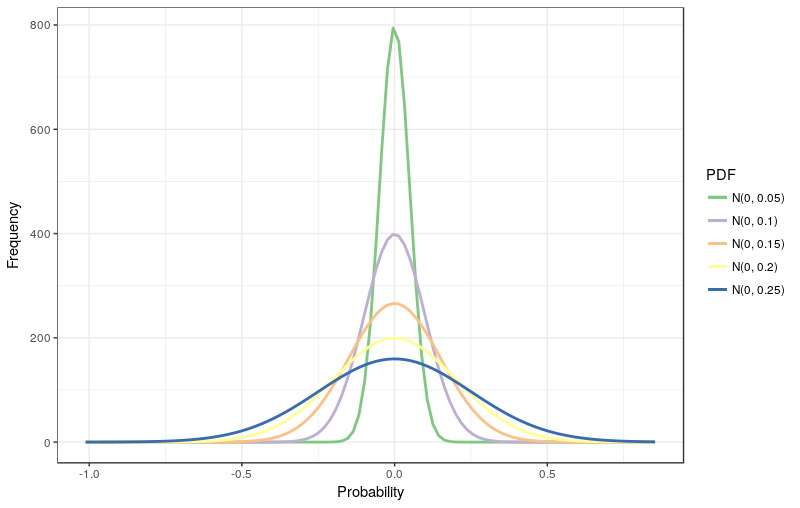
\includegraphics[width=0.8\textwidth]{img/gld_clustering/extra_images/5_gaussian.png}
    \caption{Gaussian (Normal) distributions used to generate the synthetic dataset.}
    \label{fig:5_gaussian}
\end{figure}

\begin{figure}[H]
    \centering
    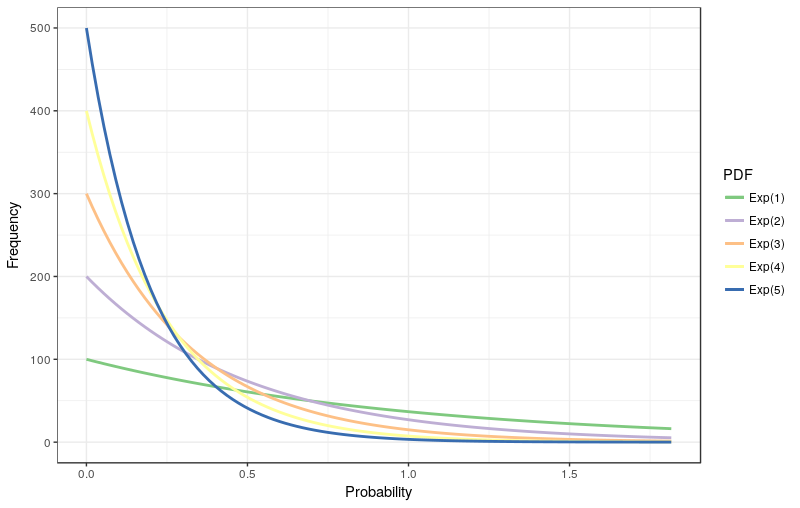
\includegraphics[width=0.8\textwidth]{img/gld_clustering/extra_images/5_exp.png}
    \caption{Exponential distributions used to generate the synthetic dataset.}
    \label{fig:5_exp}
\end{figure}

\begin{figure}[H]
    \centering
    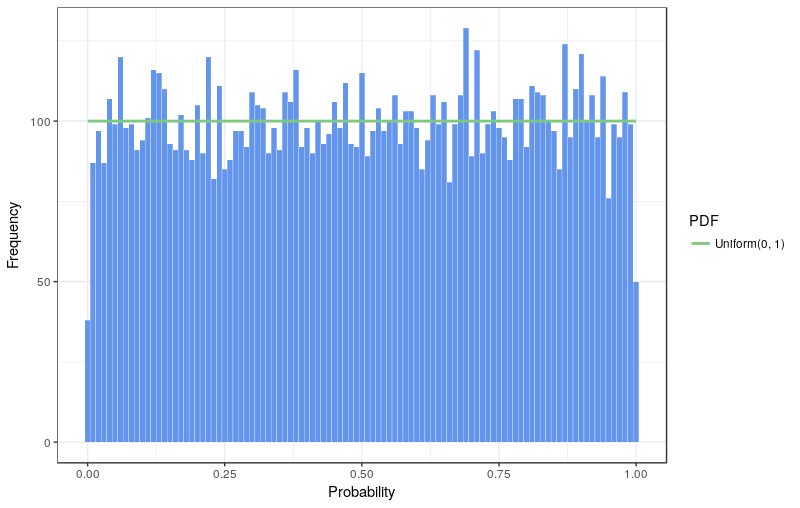
\includegraphics[width=0.8\textwidth]{img/gld_clustering/extra_images/uniform.png}
    \caption{Uniform distribution used to generate the synthetic dataset.}
    \label{fig:uniform}
\end{figure}

This dataset could be represented as a multidimensional array where for each position $x_{i}$, we have 1000 values $v_{j}$, equation \ref{eq:multi_array_datasetI}. In this case $i$ and $j$ vary from 1 to 1000 casually.

\begin{equation}\label{eq:multi_array_datasetI}
S(x_{i}, <v_{j}>) i,j=1, 2.....1000
\end{equation}

The fitting algorithm proposed in subsection \ref{sub:fitting_gld} is applied over \ref{eq:multi_array_datasetI}. The good-of-fit test return that all the \textit{GLDs} are good fit for its corresponding distribution. As a result the dataset \ref{eq:multi_array3} is genarated. 

\begin{equation}\label{eq:multi_array3}
S(x_{i}, <\lambda_{1},\lambda_{2},\lambda_{3},\lambda_{4}>)  i=1.....1000
\end{equation}

\subsection{Clustering using $\lambda_{2}$, $\lambda_{3}$ and $\lambda_{4}$}\label{syntheticI_l234}

As we mention above, our idea is to test what happen if we use a simple k-means with euclidean distance over the $\lambda_{2}$, $\lambda_{3}$ and $\lambda_{4}$ values of the \textit{GLDs}. Similar to the paper \cite{Jiang2011}, as we use 11 \textit{PDFs} to generate the synthetic dataset I, we expect that the k-mean algorithm will return 11 clusters as well (one for each distribution). Then 11 is the number we use with the k-means algorithm.

In figure \ref{fig:dataset1_l2l3l4} and table \ref{tab:dataset1_l2l3l4} the distribution of the clusters returned by the k-means is shown.

\begin{figure}[H]
    \centering
    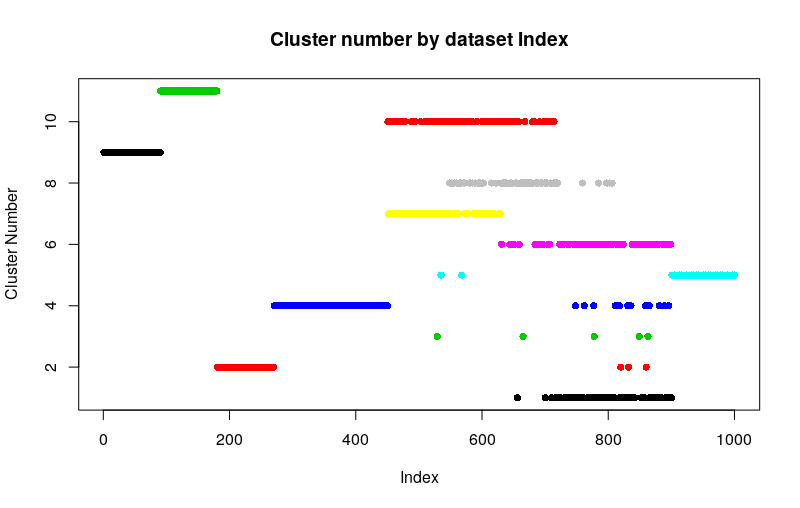
\includegraphics[width=0.8\textwidth]{img/gld_clustering/Dataset1/l2_l3_l4/intento_3/normal_exponential_uniform3.png}
    \caption{Distribution of the clusters using k-means over the $\lambda_{2}$, $\lambda_{3}$ and $\lambda_{4}$ values of the \textit{GLDs}.}
    \label{fig:dataset1_l2l3l4}
\end{figure}

\begin{table}[]
\centering
\caption{Distribution of the clusters using k-means over the $\lambda_{2}$, $\lambda_{3}$ and $\lambda_{4}$ values of the \textit{GLDs}.}
\label{tab:dataset1_l2l3l4}
\begin{tabular}{|c|c|c|}
\hline
Cluster & Type of Distribution & No. of Elements \\ \hline
1       & Exponential          & 82              \\ \hline
2       & Normal          & 93              \\ \hline
3       & Exponential          & 5             \\ \hline
4       & Normal               & 198              \\ \hline
5       & Uniform               & 102              \\ \hline
6       & Exponential               & 83             \\ \hline
7       & Exponential              & 91             \\ \hline
8       & Exponential          & 82              \\ \hline
9       & Normal          & 90               \\ \hline
10      & Exponential               & 84              \\ \hline
11      & Normal          & 90              \\ \hline
\end{tabular}
\end{table}

Remembered, the first 450 elements are normal distributions, the next 450 are exponential and the last 100 are uniform. Looking to those regions in general, the first observation is that we have 23 false positives, three in cluster 2, 18 in cluster 4 and two in cluster 5. The second observation is that, the normal distributions were grouped in 4 clusters (2, 4, 9 and 11), cluster 2 group perfectly it 90 elements with 2 false positives, clusters 9 and 11 group exactly its 90 elements each. The cluster 4 group the last 180 elements of the Normal distribution, with 18 false positives

The Uniform distribution was grouped totally in cluster 5, with two false positives as was mention above. The last observation is that the algorithm can't separate the 5 Exponential distributions, but this is not a bad result as we will show soon. 

In figures between \ref{fig:dataset1_l2l3l4_cl1} and \ref{fig:dataset1_l2l3l4_cl11} we show the \textit{PDFs} of all the distributions that belongs to the same cluster. If we take a look at figures \ref{fig:dataset1_l2l3l4_cl1}, \ref{fig:dataset1_l2l3l4_cl2}, \ref{fig:dataset1_l2l3l4_cl3}, \ref{fig:dataset1_l2l3l4_cl9}, \ref{fig:dataset1_l2l3l4_cl10} and \ref{fig:dataset1_l2l3l4_cl11} we see that the exponential distribution was well grouped. Really the problem is that the rate value of $0.05*i$ used to generate the exponential distribution does not have such a big difference between one and another.  

\begin{figure}[H]
    \centering
    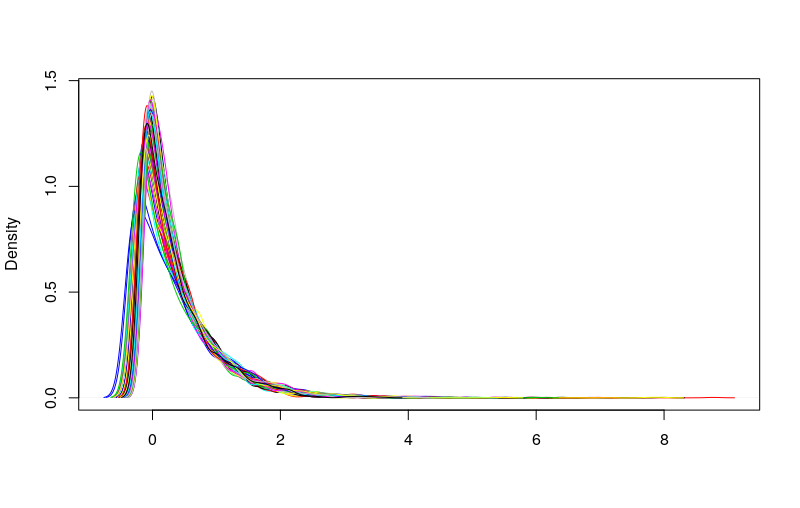
\includegraphics[width=0.8\textwidth]{img/gld_clustering/Dataset1/l2_l3_l4/intento_3/cluster1.png}
    \caption{Cluster 1 returned by the k-means over the $\lambda_{2}$, $\lambda_{3}$ and $\lambda_{4}$ values of the \textit{GLDs}, synthetic dataset I.}
    \label{fig:dataset1_l2l3l4_cl1}
\end{figure}

\begin{figure}[H]
    \centering
    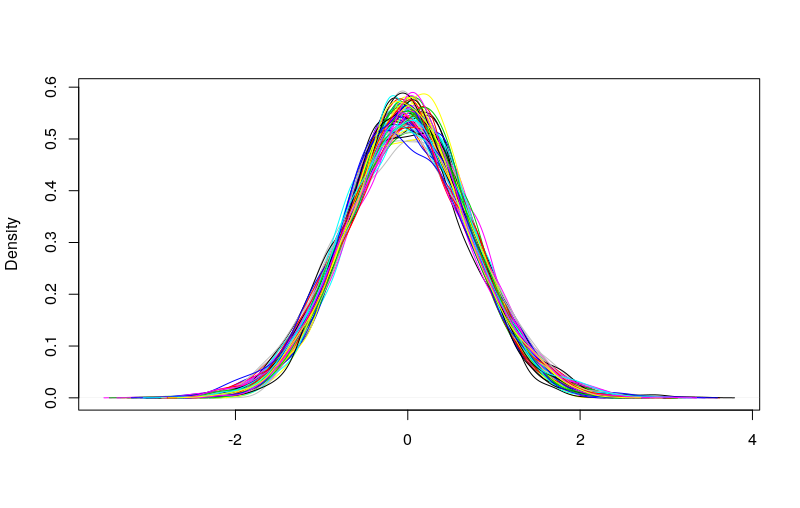
\includegraphics[width=0.8\textwidth]{img/gld_clustering/Dataset1/l2_l3_l4/cluster4.png}
    \caption{Cluster 2 returned by the k-means over the $\lambda_{2}$, $\lambda_{3}$ and $\lambda_{4}$ values of the \textit{GLDs}, synthetic dataset I.}
    \label{fig:dataset1_l2l3l4_cl2}
\end{figure}

\begin{figure}[H]
    \centering
    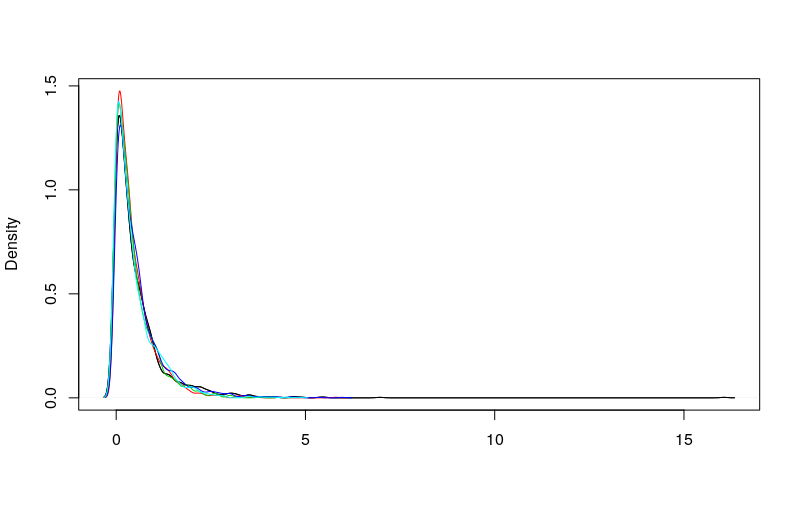
\includegraphics[width=0.8\textwidth]{img/gld_clustering/Dataset1/l2_l3_l4/intento_3/cluster3.png}
    \caption{Cluster 3 returned by the k-means over the $\lambda_{2}$, $\lambda_{3}$ and $\lambda_{4}$ values of the \textit{GLDs}, synthetic dataset I.}
    \label{fig:dataset1_l2l3l4_cl3}
\end{figure}

\begin{figure}[H]
    \centering
    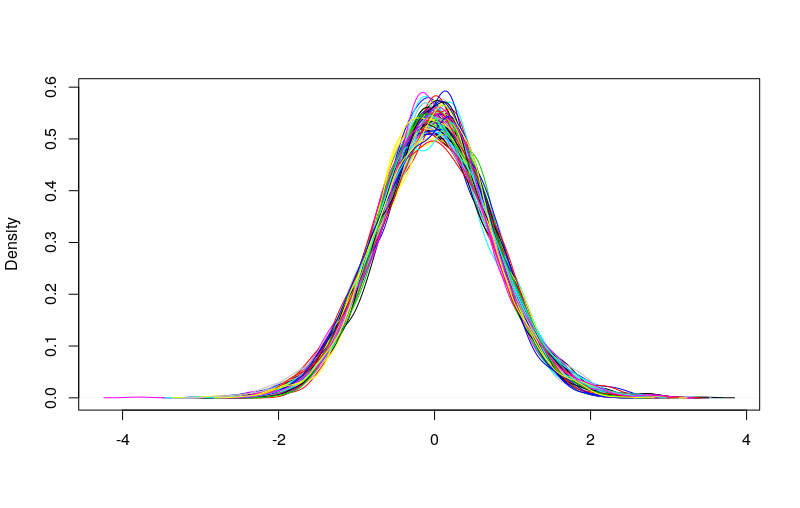
\includegraphics[width=0.8\textwidth]{img/gld_clustering/Dataset1/l2_l3_l4/cluster5.png}
    \caption{Cluster 4 returned by the k-means over the $\lambda_{2}$, $\lambda_{3}$ and $\lambda_{4}$ values of the \textit{GLDs}, synthetic dataset I.}
    \label{fig:dataset1_l2l3l4_cl4}
\end{figure}

\begin{figure}[H]
    \centering
    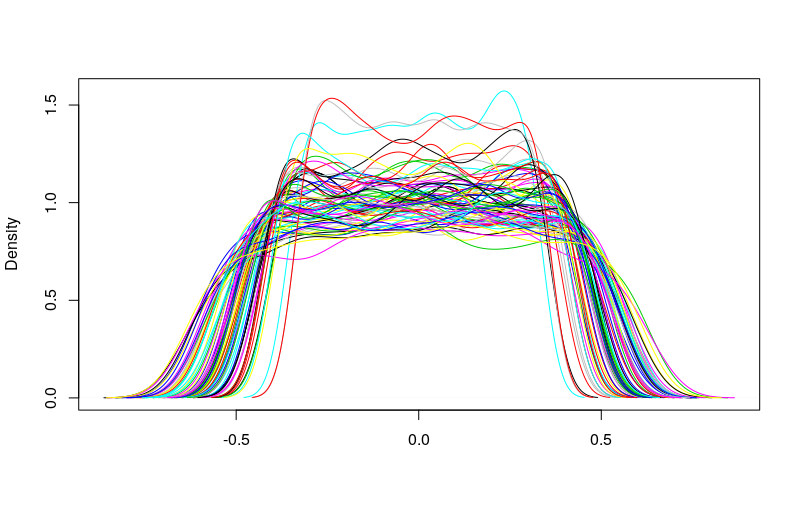
\includegraphics[width=0.8\textwidth]{img/gld_clustering/Dataset1/l2_l3_l4/cluster7.png}
    \caption{Cluster 5 returned by the k-means over the $\lambda_{2}$, $\lambda_{3}$ and $\lambda_{4}$ values of the \textit{GLDs}, synthetic dataset I.}
    \label{fig:dataset1_l2l3l4_cl5}
\end{figure}

\begin{figure}[H]
    \centering
    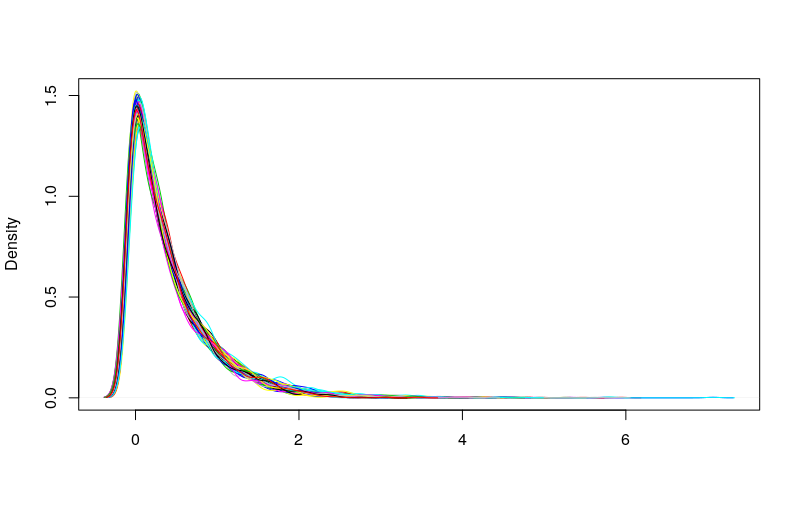
\includegraphics[width=0.8\textwidth]{img/gld_clustering/Dataset1/l2_l3_l4/intento_3/cluster6.png}
    \caption{Cluster 6 returned by the k-means over the $\lambda_{2}$, $\lambda_{3}$ and $\lambda_{4}$ values of the \textit{GLDs}, synthetic dataset I.}
    \label{fig:dataset1_l2l3l4_cl6}
\end{figure}

\begin{figure}[H]
    \centering
    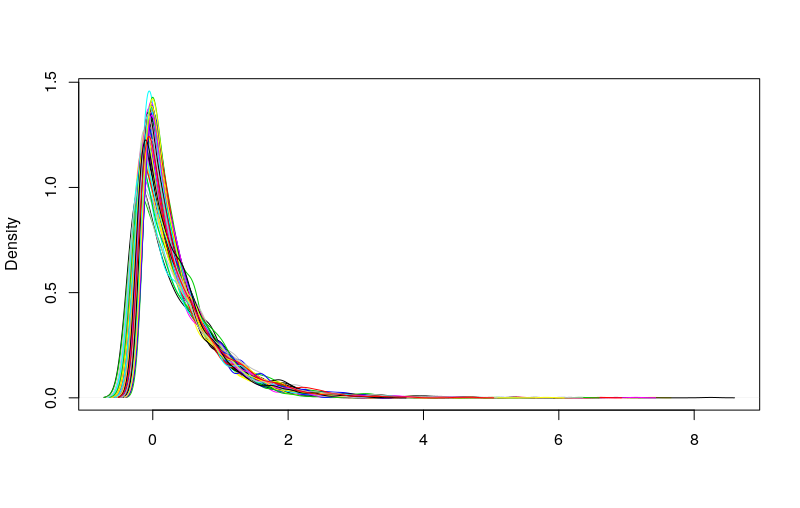
\includegraphics[width=0.8\textwidth]{img/gld_clustering/Dataset1/l2_l3_l4/intento_3/cluster7.png}
    \caption{Cluster 7 returned by the k-means over the $\lambda_{2}$, $\lambda_{3}$ and $\lambda_{4}$ values of the \textit{GLDs}, synthetic dataset I.}
    \label{fig:dataset1_l2l3l4_cl7}
\end{figure}

\begin{figure}[H]
    \centering
    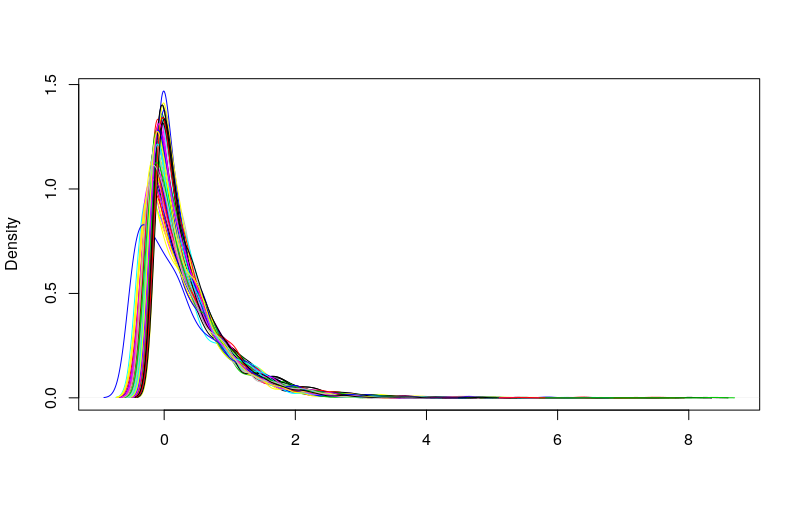
\includegraphics[width=0.8\textwidth]{img/gld_clustering/Dataset1/l2_l3_l4/intento_3/cluster8.png}
    \caption{Cluster 8 returned by the k-means over the $\lambda_{2}$, $\lambda_{3}$ and $\lambda_{4}$ values of the \textit{GLDs}, synthetic dataset I.}
    \label{fig:dataset1_l2l3l4_cl8}
\end{figure}

\begin{figure}[H]
    \centering
    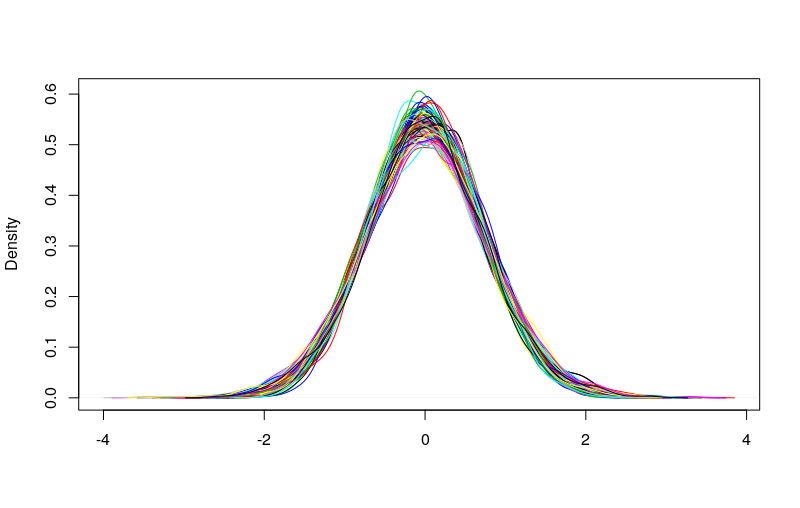
\includegraphics[width=0.8\textwidth]{img/gld_clustering/Dataset1/l2_l3_l4/intento_3/cluster9.png}
    \caption{Cluster 9 returned by the k-means over the $\lambda_{2}$, $\lambda_{3}$ and $\lambda_{4}$ values of the \textit{GLDs}, synthetic dataset I.}
    \label{fig:dataset1_l2l3l4_cl9}
\end{figure}

\begin{figure}[H]
    \centering
    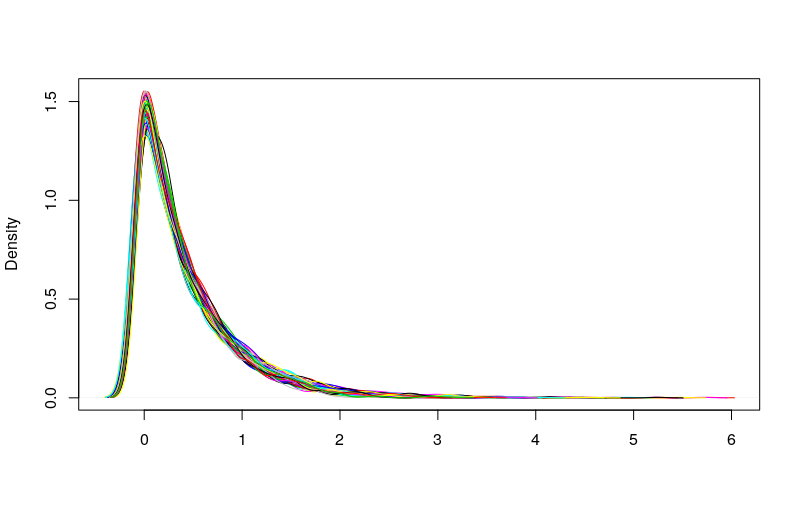
\includegraphics[width=0.8\textwidth]{img/gld_clustering/Dataset1/l2_l3_l4/intento_3/cluster10.png}
    \caption{Cluster 10 returned by the k-means over the $\lambda_{2}$, $\lambda_{3}$ and $\lambda_{4}$ values of the \textit{GLDs}, synthetic dataset I.}
    \label{fig:dataset1_l2l3l4_cl10}
\end{figure}

\begin{figure}[H]
    \centering
    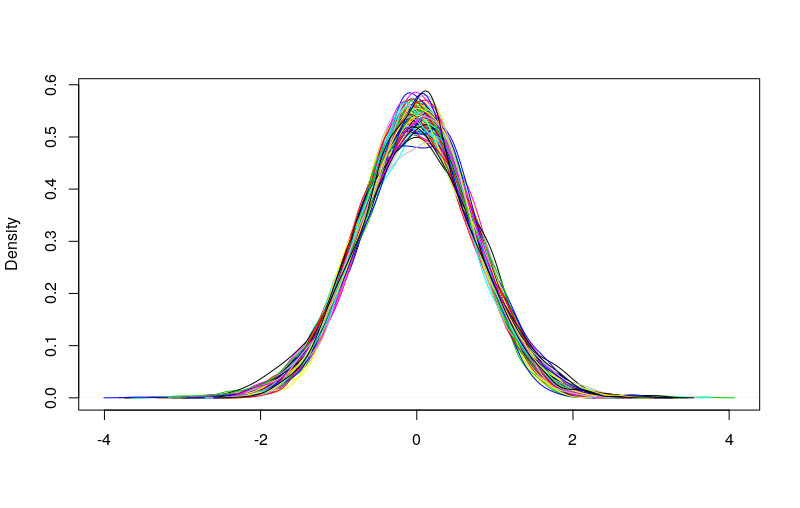
\includegraphics[width=0.8\textwidth]{img/gld_clustering/Dataset1/l2_l3_l4/intento_3/cluster11.png}
    \caption{Cluster 11 returned by the k-means over the $\lambda_{2}$, $\lambda_{3}$ and $\lambda_{4}$ values of the \textit{GLDs}, synthetic dataset I.}
    \label{fig:dataset1_l2l3l4_cl11}
\end{figure}

Another interesting result is show in figures \ref{fig:dataset1_l2l3l4_l3_l4} and \ref{fig:dataset1_l2l3l4_l3_l4_dividido}. As we can see, clusters 2, 4, 9 and 11 that represent the Normal distribution are all at the same region over the $\lambda_{3}$ and $\lambda_{4}$ space, near $\lambda_{3} = 0$ and $\lambda_{4} \in [0, 0.3]$. Similarly cluster 5, that represent the Uniform distribution is on the top left of the $\lambda_{3}$ and $\lambda_{4}$ space, $\lambda_{3} \in [0, 0.3]$ and $\lambda_{4} \in [0.7, 1.5]$. And finally the rest of the clusters that represent the Exponential distribution are distributed in the bottom of the $\lambda_{3}$ and $\lambda_{4}$ space, $\lambda_{3} \in [0.2, 7]$ and $\lambda_{4} \in [-0.1, 0.1]$. As we see in the rest of the thesis, this result is repeated in all the use cases.

\begin{figure}[H]
    \centering
    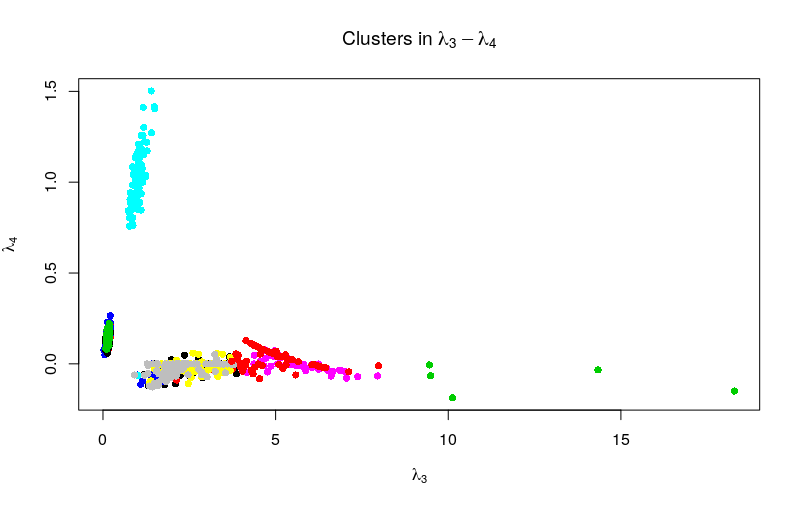
\includegraphics[width=0.8\textwidth]{img/gld_clustering/Dataset1/l2_l3_l4/intento_3/l3_l4.png}
    \caption{Distribution of the clusters over the $\lambda_{3}$ and $\lambda_{4}$ space.}
    \label{fig:dataset1_l2l3l4_l3_l4}
\end{figure}

\begin{figure}[H]
    \centering
    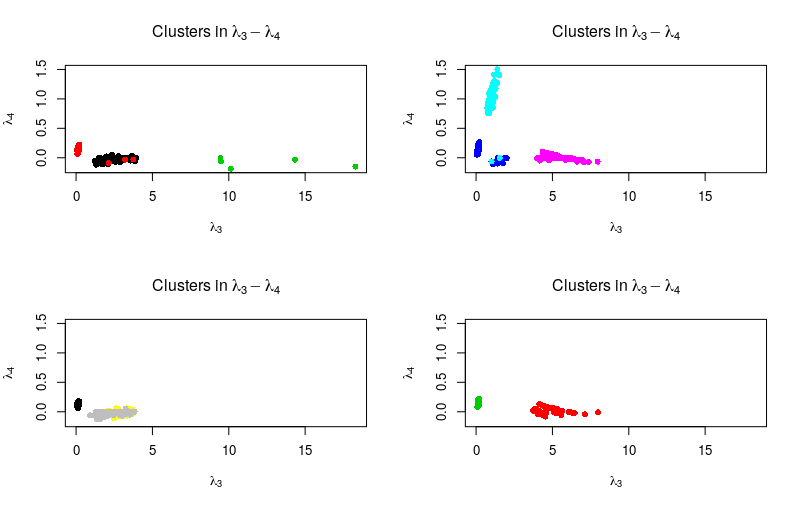
\includegraphics[width=0.8\textwidth]{img/gld_clustering/Dataset1/l2_l3_l4/intento_3/l3_l4_dividido.png}
    \caption{Distribution of the clusters over the $\lambda_{3}$ and $\lambda_{4}$ space. In the top left corner: clusters 1, 2 and 3. Top right corner: clusters 4, 5 and 6. Bottom left: clusters 7, 8 and 9. Bottom right: clusters 10 and 11.}
    \label{fig:dataset1_l2l3l4_l3_l4_dividido}
\end{figure}

\subsection{Clustering using $\lambda_{3}$ and $\lambda_{4}$}\label{syntheticI_l34}

In this section we proceed similar to section \ref{syntheticI_l234}, but the k-means algorithm run over $\lambda_{3}$ and $\lambda_{4}$. The distribution of the clusters is shown in figure \ref{fig:dataset1_l3l4} and table \ref{tab:dataset1_l3l4}.

\begin{figure}[H]
    \centering
    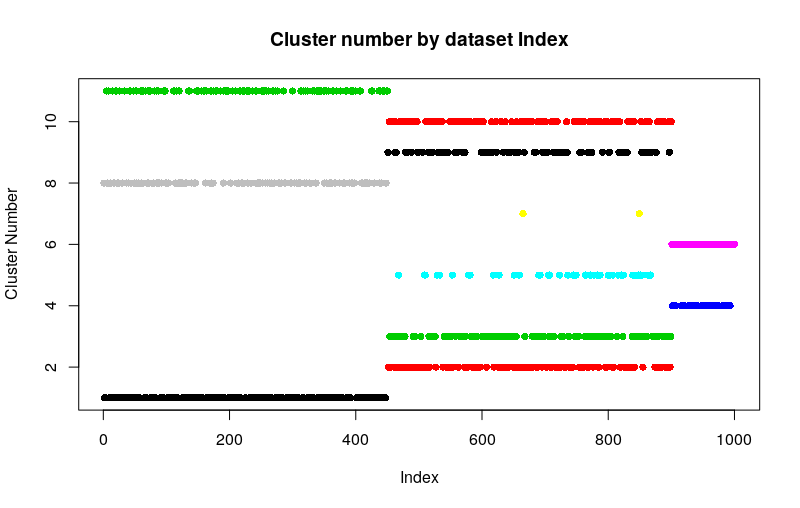
\includegraphics[width=0.8\textwidth]{img/gld_clustering/Dataset1/l3_l4/clusters_by_index.png}
    \caption{Distribution of the clusters using k-means over the $\lambda_{3}$ and $\lambda_{4}$ values of the \textit{GLDs}.}
    \label{fig:dataset1_l3l4}
\end{figure}

\begin{table}[]
\centering
\caption{Distribution of the clusters using k-means over the $\lambda_{3}$ and $\lambda_{4}$ values of the \textit{GLDs}.}
\label{tab:dataset1_l3l4}
\begin{tabular}{|c|c|c|}
\hline
Cluster & Type of Distribution & No. of Elements \\ \hline
1       & Normal          & 197              \\ \hline
2       & Exponential          & 118              \\ \hline
3       & Exponential          & 110             \\ \hline
4       & Uniform               & 35              \\ \hline
5       & Exponential               & 41              \\ \hline
6       & Uniform               & 65             \\ \hline
7       & Exponential              & 2             \\ \hline
8       & Normal          & 131              \\ \hline
9       & Exponential          & 74               \\ \hline
10      & Exponential               & 105              \\ \hline
11      & Normal          & 122              \\ \hline
\end{tabular}
\end{table}
 
 
As we don't use $\lambda_{2}$ here, is clear that the algorithm can't distinguish the distributions by its standard deviation. But, as the shape of the \textit{GLD} is defined by $\lambda_{3}$ and $\lambda_{4}$, what we expect is that the algorithm can separate the objects by type of distribution. As we see in figure \ref{fig:dataset1_l3l4} this is exactly what we get, there is no any false positive in this case, the three regions (Normal, Exponential and Uniform) are identified by the k-means.

Clusters 1, 8 and 11 group all the Normal distributions, clusters 4 and 6 group the Uniform and the rest group the Exponential.

In the $\lambda_{3}$ and $\lambda_{4}$ space the behavior is very similar at the one we get in subsection \ref{syntheticI_l234}, figures \ref{fig:dataset1_l3l4_l3_l4} and \ref{fig:dataset1_l3l4_l3_l4_dividido}. Again the distributions are concentrated near the same $(\lambda_{3}, \lambda_{4})$ values.

\begin{figure}[H]
    \centering
    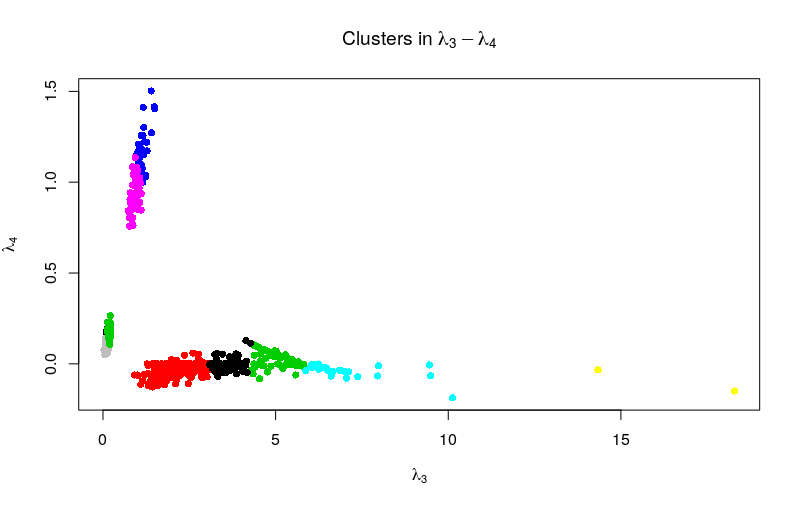
\includegraphics[width=0.8\textwidth]{img/gld_clustering/Dataset1/l3_l4/l3_l4.png}
    \caption{Distribution of the clusters over the $\lambda_{3}$ and $\lambda_{4}$ space.}
    \label{fig:dataset1_l3l4_l3_l4}
\end{figure}

\begin{figure}[H]
    \centering
    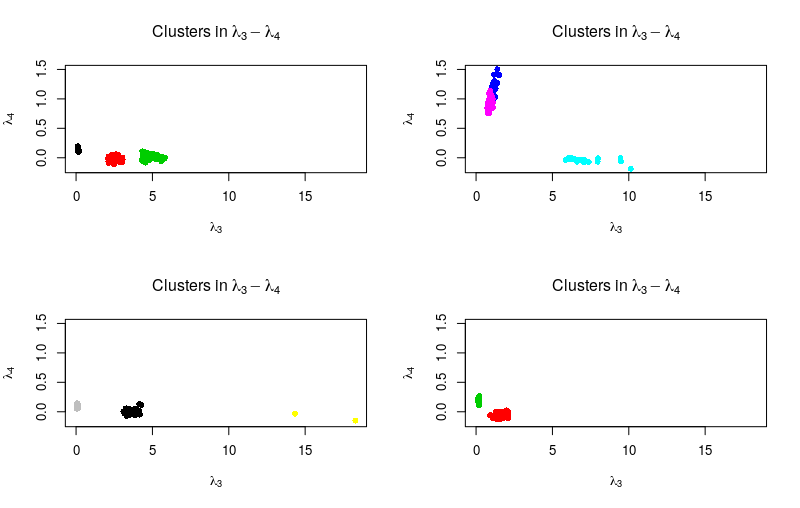
\includegraphics[width=0.8\textwidth]{img/gld_clustering/Dataset1/l3_l4/l3_l4_dividido.png}
    \caption{Distribution of the clusters over the $\lambda_{3}$ and $\lambda_{4}$ space. In the top left corner: clusters 1, 2 and 3. Top right corner: clusters 4, 5 and 6. Bottom left: clusters 7, 8 and 9. Bottom right: clusters 10 and 11.}
    \label{fig:dataset1_l3l4_l3_l4_dividido}
\end{figure}

%\subsection{Effectiveness of the Clustering}

\section{Synthetic Data II}\label{sec:synthetic_II}
The second synthetic dataset is similar to the first one, here we include 5 Gamma distributions, between the Exponential and the Uniform, figure \ref{fig:5_gamma}. The shape of the Gamma distribution is $i$, with $i=1, 2, 3, 4, 5$. This dataset have 1450 objects, where the first 450 were sampled from a Gaussian distributions, the next 450 from an Exponential, the next 450 are Gamma, and the last 100 from a Uniform distribution. As we use 16 different distributions, this is the number of clusters to be used with the k-means algorithm. 

\begin{figure}[H]
    \centering
    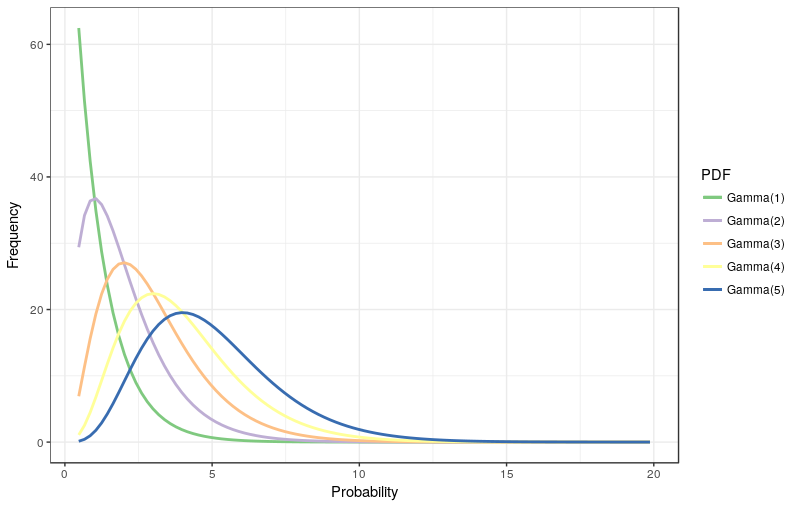
\includegraphics[width=0.8\textwidth]{img/gld_clustering/extra_images/5_gamma.png}
    \caption{Gamma distributions used to generate the synthetic dataset.}
    \label{fig:5_gamma}
\end{figure}

Similar to the dataset I, the fitting algorithm proposed in subsection \ref{sub:fitting_gld} is applied over dataset II. The good-of-fit test return that all the \textit{GLDs} are good fit for its corresponding distribution.

\subsection{Clustering using $\lambda_{2}$, $\lambda_{3}$ and $\lambda_{4}$}\label{syntheticII_l234}

The distribution of the clusters returned by the k-means algorithm is shown in figure \ref{fig:dataset2_l2l3l4} and table \ref{tab:dataset2_l2l3l4}.

\begin{figure}[H]
    \centering
    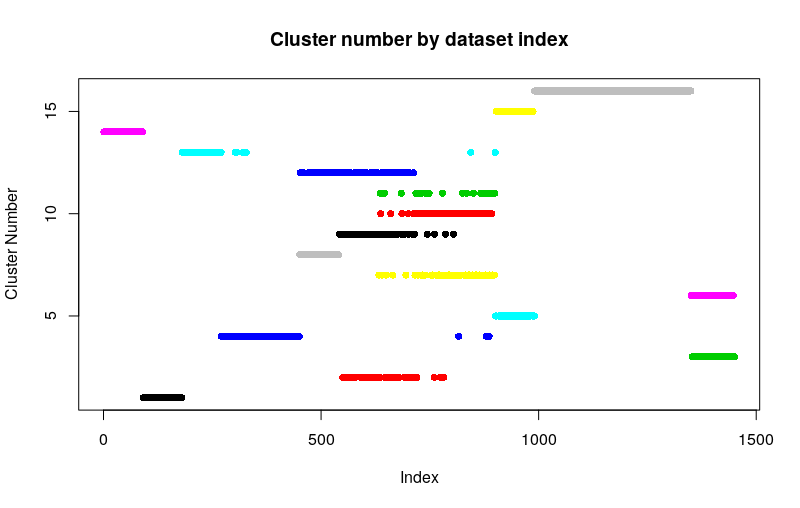
\includegraphics[width=0.8\textwidth]{img/gld_clustering/Dataset2/nuevo/clusters_by_index.png}
    \caption{Distribution of the clusters using k-means over the $\lambda_{2}$, $\lambda_{3}$ and $\lambda_{4}$ values of the \textit{GLDs}.}
    \label{fig:dataset2_l2l3l4}
\end{figure}

\begin{table}[]
\centering
\caption{Distribution of the clusters using k-means over the $\lambda_{2}$, $\lambda_{3}$ and $\lambda_{4}$ values of the \textit{GLDs}.}
\label{tab:dataset2_l2l3l4}
\begin{tabular}{|c|c|c|}
\hline
Cluster & Type of Distribution & No. of Elements \\ \hline
1       & Normal          & 90              \\ \hline
2       & Exponential          & 44              \\ \hline
3       & Uniform          & 45             \\ \hline
4       & Normal               & 179              \\ \hline
5       & Gamma               & 60             \\ \hline
6       & Uniform               & 55            \\ \hline
7       & Exponential              & 87            \\ \hline
8       & Exponential          & 58              \\ \hline
9       & Exponential          & 67               \\ \hline
10      & Exponential               & 74              \\ \hline
11      & Exponential          & 25              \\ \hline
12       & Exponential              & 90             \\ \hline
13       & Normal          & 96              \\ \hline
14       & Normal          & 90              \\ \hline
15      & Gamma               & 30              \\ \hline
16      & Gamma          & 360              \\ \hline
\end{tabular}
\end{table}

In general the results are very similar to the results of the section \ref{sec:synthetic_I}, but we get less false positives, 5 in total. 3 false positives in cluster 4 and 2 false positves in cluster 13. The normal distribution was groping again in for clusters: 1, 4, 13 and 14. The uniform distribution was grouping in clusters 3 and 6 without false positives. The gamma distribution introduced here was grouped in clusters 5, 15 and 16, without false positives. And finally the rest of the clusters are for the exponential distribution.

The projection of the clusters over the $\lambda_{3}$ and $\lambda_{4}$ space is show in figure \ref{fig:dataset2_l2l3l4_l3_l4}. The two clusters of the uniform distribution are located again in the top-left region of the figure. The normal distribution is located in the same place, near $\lambda_{3} = 0$ and $\lambda_{4} \in [0, 0.3]$. The exponential distribution is distributed in the bottom of the $\lambda_{3}$ and $\lambda_{4}$ space. The gamma distribution is overlapped together with the normal distribution.

\begin{figure}[H]
    \centering
    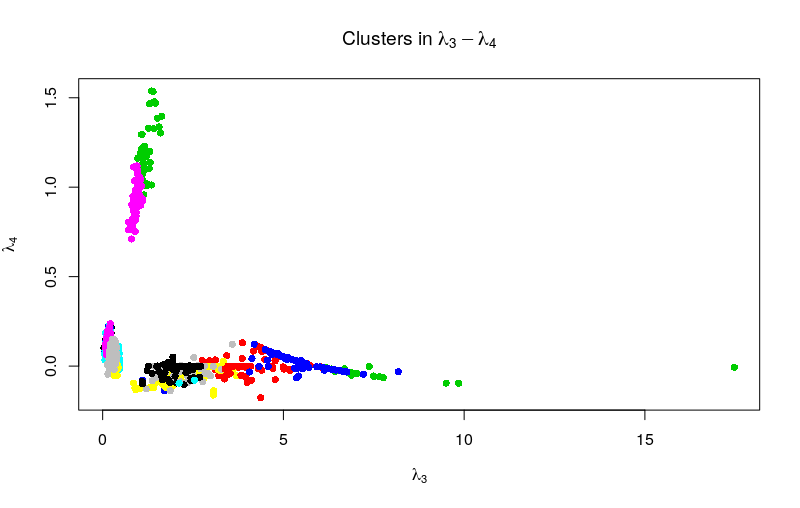
\includegraphics[width=0.8\textwidth]{img/gld_clustering/Dataset2/nuevo/l3_l4.png}
    \caption{Distribution of the clusters over the $\lambda_{3}$ and $\lambda_{4}$ space.}
    \label{fig:dataset2_l2l3l4_l3_l4}
\end{figure}

%\begin{figure}[H]
%    \centering
%    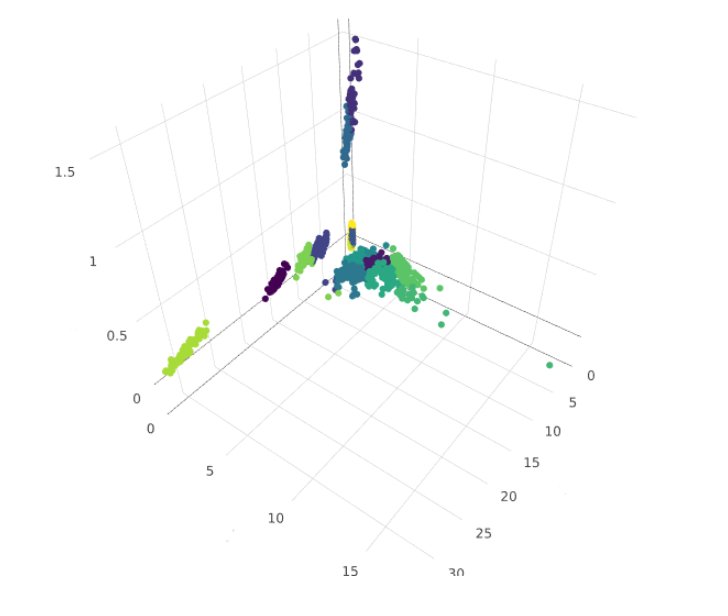
\includegraphics[width=0.8\textwidth]{img/gld_clustering/Dataset2/nuevo/l2_l3_l4_cortado.png}
%    \caption{Distribution of the clusters over the $\lambda_{2}$,  $\lambda_{3}$ and $\lambda_{4}$ space.}
%    \label{fig:dataset2_l2l3l4_l2_l3_l4}
%\end{figure}

\subsection{Clustering using $\lambda_{3}$ and $\lambda_{4}$}\label{syntheticI_l34}

The distribution of the clusters returned by the k-means when using the values of $\lambda_{3}$ and $\lambda_{4}$ to group the second synthetic dataset are shown in figure \ref{fig:dataset2_l3l4} and table \ref{tab:dataset2_l3l4}.
 
A few false positives are observed in clusters 5, 6 and 12, but nothing to worry about. Again the regions of the four distribution families are perfectly separated by the algorithm. 
 
\begin{table}[]
\centering
\caption{Distribution of the clusters using k-means over the $\lambda_{3}$ and $\lambda_{4}$ values of the \textit{GLDs}.}
\label{tab:dataset2_l3l4}
\begin{tabular}{|c|c|c|}
\hline
Cluster & Type of Distribution & No. of Elements \\ \hline
1       & Exponential          & 64              \\ \hline
2       & Exponential          & 126              \\ \hline
3       & Exponential          & 1             \\ \hline
4       & Exponential               & 57              \\ \hline
5       & Gamma               & 83             \\ \hline
6       & Normal               & 139            \\ \hline
7       & Uniform              & 67            \\ \hline
8       & Gamma          & 148              \\ \hline
9       & Gamma          & 108               \\ \hline
10      & Exponential               & 75              \\ \hline
11      & Exponential          & 80              \\ \hline
12       & Normal              & 112             \\ \hline
13       & Exponential          & 44              \\ \hline
14       & Normal          & 201              \\ \hline
15      & Gamma               & 112              \\ \hline
16      & Uniform          & 33              \\ \hline
\end{tabular}
\end{table}
 
 \begin{figure}[H]
    \centering
    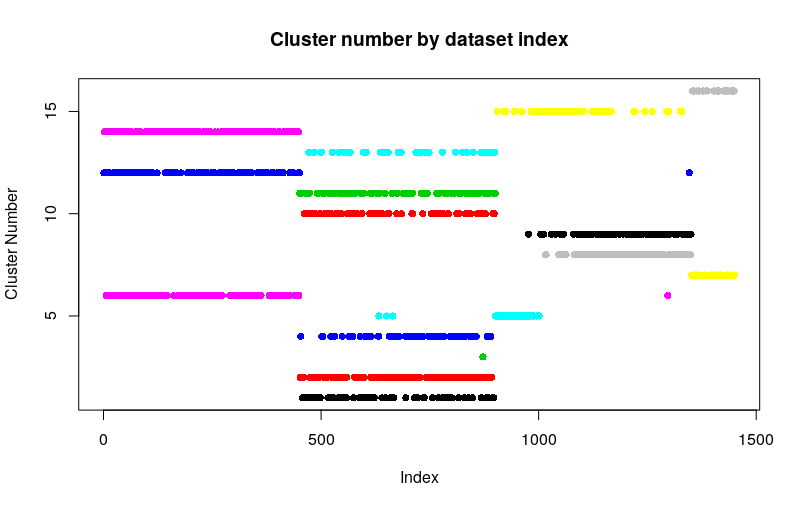
\includegraphics[width=0.8\textwidth]{img/gld_clustering/Dataset2/nuevo/l3_l4/clusters_by_index.png}
    \caption{Distribution of the clusters using k-means over the $\lambda_{2}$, $\lambda_{3}$ and $\lambda_{4}$ values of the \textit{GLDs}.}
    \label{fig:dataset2_l3l4}
\end{figure}

The projection of the clusters over the $\lambda_{3}$ and $\lambda_{4}$ space is show in figure \ref{fig:dataset2_l3l4_l3_l4}.

\begin{figure}[H]
    \centering
    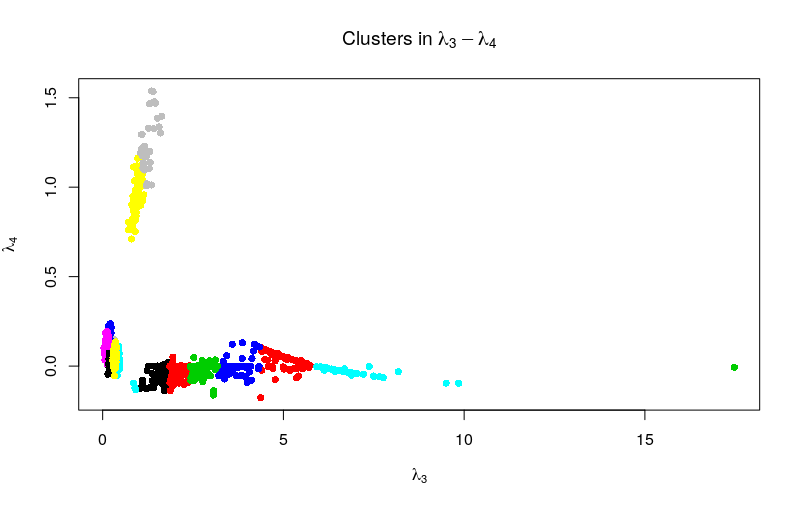
\includegraphics[width=0.8\textwidth]{img/gld_clustering/Dataset2/nuevo/l3_l4/l3_l4.png}
    \caption{Distribution of the clusters over the $\lambda_{3}$ and $\lambda_{4}$ space.}
    \label{fig:dataset2_l3l4_l3_l4}
\end{figure}

%\subsection{Effectiveness of the Clustering}

\section{Conclusions}\label{sec:conclusions}

In this chapter, we explore clustering uncertain data based on the similarity between their distributions. The idea is to answer the research question 1 \textit{"how to group the output of the UQ process based on the similarity of the uncertainty?"}. Different to the approaches reported in the literature, we propose the use of a k-means algorithm with euclidean distance over the $\lambda_{2}$, $\lambda_{3}$ and $\lambda_{4}$ space of the \textit{GLD}. 

The approach was tested over two synthetic datasets and the results of the  test were exactly what we expect.


%\section{Ideas por si son necesarias}
%
%\subsection{The Gaussian (Normal) Distribution}
%The Gaussian (Normal) distribution is probably the most used and also the most well-known distribution. Many groups follow this type of pattern. That's why it's widely used in business, statistics and in government bodies like the FDA:
%\begin{itemize}
%\item Heights of people.
%\item Measurement errors.
%\item Blood pressure.
%\item Points on a test.
%\item IQ scores.
%\item Salaries.
%\end{itemize}
%
%The PDF of the Normal Distribution is represented in equation \ref{eq:gaussian_distribution}
%
%\begin{equation}\label{eq:gaussian_distribution}
%f(x) = \frac{1}{{ \sqrt {2\pi \sigma} }}e^{{{ - \left( {x - \mu } \right)^2 } \mathord{\left/ {\vphantom {{ - \left( {x - \mu } \right)^2 } {2\sigma ^2 }}} \right. \kern-\nulldelimiterspace} {2\sigma ^2 }}}
%\end{equation}
%
%where:
%\begin{itemize}
%\item $\mu$ is the mean or expectation of the distribution (and also its median and mode),
%\item $\sigma$ is the standard deviation, and
%\item $\sigma^2$ is the variance.
%\end{itemize}
%
%To generate a synthetic normal distribution we need to specify the number of elements we want (e.g. 1000) and the mean and standard deviation. In \textit{R} for example we can use a function \textbf{\textit{rnorm(1000, 0, 2)}} to generate 1000 elements of a normal distribution with mean $\mu = 0$ and standard deviation $\sigma = 2$, figure \ref{fig:normal_sample}.
%
%\begin{figure}[H]
%    \centering
%    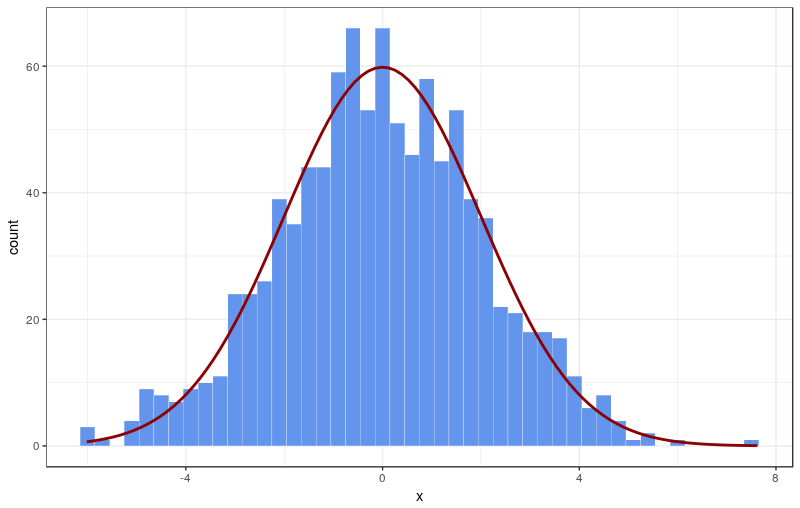
\includegraphics[width=0.8\textwidth]{img/gld_clustering/extra_images/normal_0_2.png}
%    \caption{Normal distribution generated using the \textit{R} function \textbf{\textit{rnorm(1000, 0, 2)}} with mean $\mu = 0$ and standard deviation $\sigma = 2$.}
%    \label{fig:normal_sample}
%\end{figure}
%
%\subsection{The Exponential Distribution}
%\begin{equation}\label{eq:exponential_distribution}
%  f(x) =
%  \begin{cases}
%    \lambda e^{-\lambda x} & \text{$x >= 0 $} \\
%    0 & \text{$x < 0$}
%  \end{cases}
%\end{equation}
%
%\begin{figure}[H]
%    \centering
%    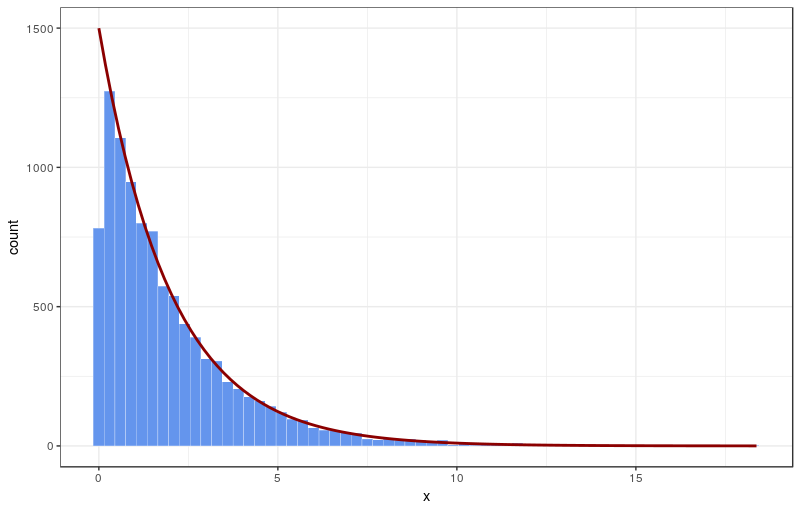
\includegraphics[width=0.8\textwidth]{img/gld_clustering/extra_images/exp_05.png}
%    \caption{Exponential distribution generated using the \textit{R} function \textbf{\textit{rexp(1000, 0.5)}} with rate $\lambda = 0.5$.}
%    \label{fig:normal_sample}
%\end{figure}
%
%\subsection{The Uniform Distribution}
%\begin{equation}\label{eq:uniform_distribution}
%  f(x) =
%  \begin{cases}
%    \frac{1}{b-a} & \text{$a < x < b$} \\
%    0 & \text{$x < a$ or $x > b$}
%  \end{cases}
%\end{equation}
%
%\begin{figure}[H]
%    \centering
%    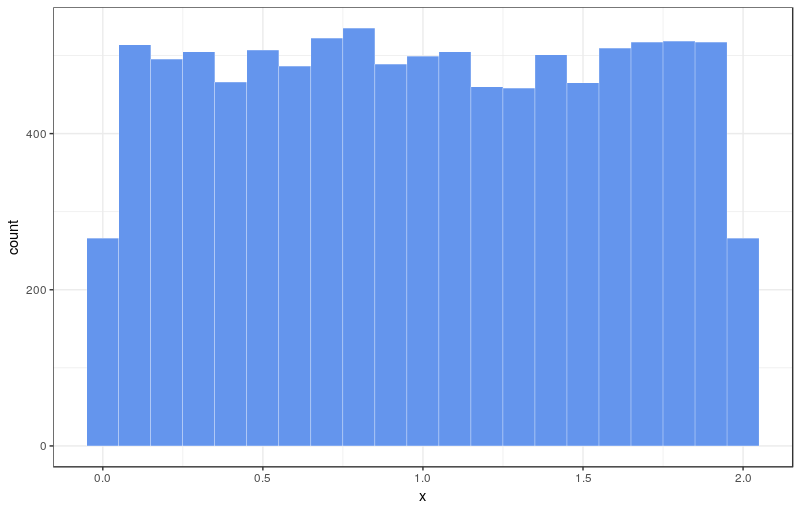
\includegraphics[width=0.8\textwidth]{img/gld_clustering/extra_images/unif_0_2.png}
%    \caption{Uniform distribution generated using the \textit{R} function \textbf{\textit{runif(1000, 0, 2)}} in the interval $[0, 2]$.}
%    \label{fig:normal_sample}
%\end{figure}
%
%\subsection{The Gamma Distribution}
%\begin{equation}\label{eq:gamma_distribution}
%  f(x) =
%  \begin{cases}
%    \frac{x^{\alpha-1}e^{\frac{-x}{\theta}}}{\Gamma(\alpha)\theta^{\alpha}} & \text{$x >= 0 $} \\
%    0 & \text{$x < 0$}
%  \end{cases}
%\end{equation}
%
%\begin{figure}[H]
%    \centering
%    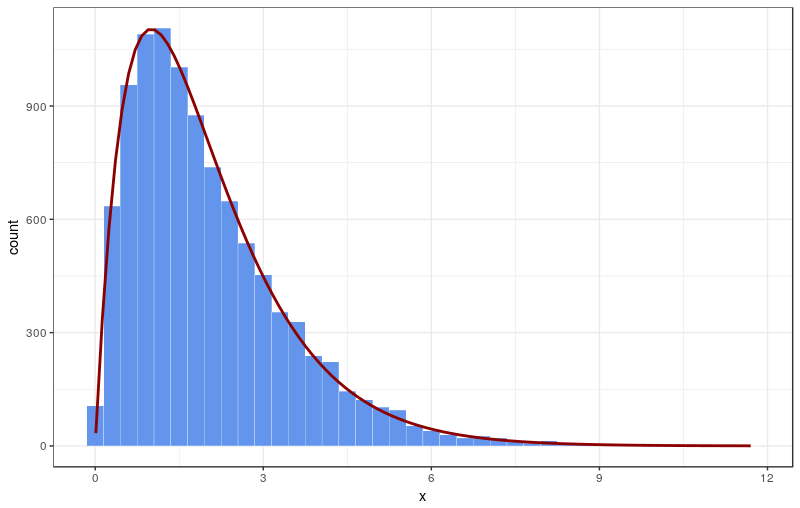
\includegraphics[width=0.8\textwidth]{img/gld_clustering/extra_images/gamma_2.png}
%    \caption{Gamma distribution generated using the \textit{R} function \textbf{\textit{rgamma(1000, 2)}} with shape $\alpha = 2$.}
%    \label{fig:normal_sample}
%\end{figure}
